%%
%% This is file `./samples/longsample.tex',
%% generated with the docstrip utility.
%%
%% The original source files were:
%%
%% apa7.dtx  (with options: `longsample')
%% ----------------------------------------------------------------------
%% 
%% apa7 - A LaTeX class for formatting documents in compliance with the
%% American Psychological Association's Publication Manual, 7th edition
%% 
%% Copyright (C) 2019 by Daniel A. Weiss <daniel.weiss.led at gmail.com>
%% 
%% This work may be distributed and/or modified under the
%% conditions of the LaTeX Project Public License (LPPL), either
%% version 1.3c of this license or (at your option) any later
%% version.  The latest version of this license is in the file:
%% 
%% http://www.latex-project.org/lppl.txt
%% 
%% Users may freely modify these files without permission, as long as the
%% copyright line and this statement are maintained intact.
%% 
%% This work is not endorsed by, affiliated with, or probably even known
%% by, the American Psychological Association.
%% 
%% ----------------------------------------------------------------------
%% 
\documentclass[man]{apa7}

\usepackage{lipsum}

\usepackage[american]{babel}
\usepackage{caption}%
\usepackage{amsmath}
\usepackage{amssymb}


\usepackage{lscape}%
\usepackage{csquotes}%
\usepackage{subfigure}%
\usepackage{graphicx}%
\usepackage{longtable}
\usepackage{array}%
\usepackage{multirow}%
\usepackage{csquotes}
\usepackage[style=apa,sortcites=true,sorting=nyt,backend=biber]{biblatex}
\DeclareLanguageMapping{american}{american-apa}
\addbibresource{bibliography.bib}

\title{Political Party Control and Intergovernmental Transfer: a Longitudinal Study}
\shorttitle{Political Party Contril and Intergovernmental Transfer: a Longitudinal Study}

\author{Yan Hao}

\affiliation{Pennsylvania State University\\School of Public Affairs}

\leftheader{Weiss}

\abstract{Intergovernmental transfer (IGT) programs are typically disbursed either through a competitive process or a predetermined formula. Formula grants are allocated among recipients based on factors stipulated in enabling legislation or administrative regulations, such as population, median household income, per capita income, poverty rates, and the number of miles driven. In contrast, the federal government possesses the authority to allocate competitive grants.

The purpose of this study is to investigate how the distribution of political party control affects IGTs by analyzing longitudinal IGT data from 18 states, utilizing a fixed-effect model. The considered effects of political party control include (1) unified federal government, (2) the specific party in control, (3) the power distribution between the administrative and legislative branches, and (4) the alignment between the federal and state governments. Examining these effects is crucial due to the escalating hostility between the Democratic and Republican parties. The potential impact of political party control on IGT grants distribution warrants thorough exploration.

In this paper, we derive implications regarding the grant-in-aid budgeting process and the role of political parties in this policymaking process.} %chatgpt checked

\keywords{intergovernmental transfer, partisian , longitudinal study}

\authornote{
   \addORCIDlink{Yan Hao}{0009-0000-6310-3988}

  Correspondence concerning this article should be addressed to Yan Hao, School of Public Affairs, Public Administration, Pennsylvania State University Harrisburg, 777 W Harrisburg Pike, Middletown, PA
  17057.  E-mail: yjh5219@psu.edu}


\begin{document}
\maketitle

\section{Introduction}


In United States, approximately \$700 billion, constituting almost 20\% of federal revenues, is annually allocated across various state and local government grant programs \parencite{rosenstiel2021congressional}. Consequently, the mechanism for distributing intergovernmental transfers has long been a compelling topic in public finance.

In the US federal fiscal system, grants-in-aid programs are generally categorized along two dimensions: the level of restrictions attached to the awards and the administrative procedures governing the award process. In terms of restrictions, intergovernmental Transfers (IGT) can be classified into categorical grants, block grants, and general revenue sharing grants. Categorical grants encompass formula categorical grants, open-ended reimbursement categorical grants, and project categorical grants. Project categorical grants involve a relatively strict set of activities tied to a specific purpose. Block grants are allocated to fund specific programs but impose relatively few restrictions, notably lacking a specific purpose attached to the recipient's spending. General revenue sharing grants carry the least amount of restrictions, allowing expenditures for any purpose not prohibited by federal or state law.

According to a Congressional Research Service report, there are approximately 600 grant-in-aid programs, with categorical grants constituting about 95 percent of the programs and more than 80 percent of total grant outlays \parencite{dilger2015federal}. The intergovernmental transfer categories are summarized in Table \ref{igtkinds}.%%%chatgpt checked%%%

\begin{table}[H]
  \centering
  \caption{Divide Grants by level of Restriction Attached}
  \begin{tabular}{ccc}
    \toprule
    \multicolumn{3}{c}{Level of Restriction}                                   \\
    \midrule
    Low Restriction           & Medium Restriction & High Restriction          \\
    \midrule
    Formula Categorical Grant & Block Grant        & Project Categorical Grant \\
    Open-ended Reimbursement  &                    &                           \\
    General Revenue Sharing   &                    &                           \\
    \bottomrule
  \end{tabular}%
  \label{igtkinds}%
\end{table}%

In terms of the administrative procedures governing the awards, grants can be categorized into three types: project grants (or competitive grants), formula grants, and reimbursement grants. Competitive grants require states to apply by submitting a request and obtain the grants through a competitive process. They aim to enhance funding allocation efficiency by encouraging grantees to seek funds for well-planned and exemplary projects.

Formula grants are distributed to states through mathematical formulas determined by social characteristics within the jurisdiction. The factors in the formula typically depend on the grants' intention, with common factors including population, poverty level, income per capita, unemployment rate, enrollment in public schools, etc.

Reimbursement grants award state and local governments in the form of reimbursement for a specific percentage of state and local spending on a program, without a specific limit on the reimbursement amount. Reimbursement grants can be further classified into open and closed-ended reimbursement grants. The matching mechanism in reimbursement grants is a significant consideration in public economic literature when evaluating distortion effects. In matching grants, the federal government reimburses a specific ratio for each dollar of state and local expenditure. Based on whether the federal government sets a cap on the matching grants, they can be divided into open-ended matching grants and closed-ended grants. These grant types are listed in Table \ref{Table 1.4}.%%%chatgpt checked%%%
\begin{table}[htbp]
  \centering
  \caption{Divide Grants by Form of Administrative Procedure}
  \begin{tabular}{clc}
    \toprule
    \multicolumn{3}{c}{Form of Administrative Procedure}                                                                                                     \\
    \midrule
    \multicolumn{1}{p{9.645em}}{ Submitting Request} & \multicolumn{1}{p{10.285em}}{               By Formula} & \multicolumn{1}{p{10.855em}}{Reimbursement} \\
    \midrule
    \multicolumn{1}{l}{Competitive Grants}           & Formula grants                                          & Project Categorical Grant                   \\
                                                     & Formula-project grants                                  &                                             \\
    \bottomrule
  \end{tabular}%
  \label{Table 1.4}%
\end{table}%


Investigations into the distribution of intergovernmental transfers generally treat the distribution results as bargaining outcomes among members of a specific decision-making group. Typically, these investigations do not consider subjective biases, despite the widely recognized significance of factors such as partisan alignment between central and subnational governments, competition among different branches, government popularity, and others\parencite{tellier2006public,petry1999electoral,balla2002partisanship,bickers2000congressional}.

This paper presents an empirical investigation into the effects of partisanship and different branches in intergovernmental transfer distribution.

\section{Literature Review}
\subsection{Review on Theoretical Investigation}

The distribution of grants in democratic countries is considered a bargaining game among decision-making groups, such as committees, congress, or houses, depending on which group is the decisive institution. Four assumptions are crucial in simulating the grants distribution bargaining using bargaining models: the recognition rule, voting rule, amendment rule, and money-distribution rule.

The recognition rule determines how to select an agenda setter to make the initial proposal, with most literature assuming the random recognition rule. This means that $n$ members among the decision-making institution have equal probabilities of being chosen to make the initial proposal \parencite{kalandrakis2004three,anesi2015bargaining,diermeier2011legislative,rosenstiel2021congressional}.

The voting rule establishes the standard for passing the proposal, with the majority rule and unanimous voting rule being common. The amendment rule places constraints on making amendments, ranging from the closed rule (allowing no amendments) to the open rule (allowing any and all germaine amendments).

Finally, the grants-type rule determines how grants could be manipulated by decision-making institutions, with some scholars assuming direct decisions on the number of receivers, referred to as "earmarks" or "pork barrel" spending models. The mechanism of intergovernmental transfer distribution, which accounts for nearly 20 percent of overall federal revenues, is a compelling topic in the public finance area, particularly in democratic countries like the United States.%%chatgpt checked%%%


\Textcite{baron1989bargaining} laid the foundation for subsequent analyses of bargaining models. They made several important assumptions, such as random recognition, majority voting rule, and earmarks rule. Their work, as well as the generalization by \Textcite{banks2006general}, demonstrates that legislators with agenda-setting power tend to receive a disproportionate share of funding. In addition, the equilibrium is characterized by funds flowing only to legislators in the winning coalition, with no funds allocated to those outside of it. Furthermore, they found that when proposals are brought up under a closed rule, the winning coalition is minimized, leading to the maximization of benefits for the members of the winning coalition.

\Textcite{baron1989bargaining}'s work is pioneering in the field of grants distribution, but its heavy reliance on the "earmarks" assumption limits its explanatory power in the actual political environment. \Textcite{martin2018dividing} addresses this issue by modifying the assumptions of the model. Specifically, he restricts the power of decision-making members to only determine the factors in the formula rather than the specific numbers. This modification is a significant step towards reflecting the realities of political and administrative life.

Martin's model generates different conclusions compared to Baron and Ferejohn's work. In contrast to the latter, Martin predicts oversized winning coalitions and the emergence of persistent winning blocs. Additionally, he demonstrates that when bargaining over a low-dimensional formula, legislators have limited ability to target funds to specific districts, a prediction supported by empirical evidence. For instance, Martin analyzed existing formula grants and found that 95\% of the formulas have fewer than 5 variables, indicating limited bargaining dimensions for members. Consequently, some jurisdictions can be free-riders, even if they are not part of the winning coalition. Martin predicts positive distribution outside the winning coalition as a consequence.%%%%%%%%%%%%chatgpt checked%%%

\subsection{Review on Empirical Investigation}

Beyond the introductory considerations of intergovernmental transfers in theoretical investigations, a primary challenge in their distribution lies in the political environment where such allocations transpire. The apportionment of intergovernmental transfers is often susceptible to the influence of individual political agendas, potentially compromising the intended structure of distribution procedures. A more in-depth inquiry is imperative to comprehend the mechanisms governing the distribution of intergovernmental grants. For instance, in the context of the United States, it is crucial to examine the divergent impacts when different political parties prevail in negotiations and discern the role of partisanship within subnational governments.

In conclusion, the intricate interplay of politics significantly influences the allocation of intergovernmental transfers, warranting a comprehensive understanding of the distribution mechanisms, particularly in the American context.

Given the pivotal role of intergovernmental transfers in the U.S. federal system, the impact of politics on their allocation can be excessively burdensome. Various anecdotal examples underscore this phenomenon, including the protracted efforts of Robert Carlyle Byrd to channel federal spending to his home state, West Virginia, spanning two decades. One notable instance of Byrd's influence manifests in the formulation of a new distribution formula for a trust fund surplus, proposed by him during the 1992-1997 authorization negotiations. This recalibrated formula predominantly favored states with elevated state gasoline tax rates and diminished per capita income, with West Virginia standing as a pertinent beneficiary.%%%%chatgpt checked%%%

\textcite{markusen1981benefits} conducted a descriptive study analyzing three distinct shifts in the distribution of federal grants to cities during the 1960s and 1970s. The research revealed a substantial increase in federal grants during this period, with northeastern and midwestern cities benefiting the most from 1965-1972, southern and western cities from 1972-1975, and a slight return in favor of the first group from 1975-1978. These variations can be partially attributed to the political landscape. \textcite{stegarescu2006decentralised} explains that the degree of Intergovernmental Transfer (IGT) decentralization is influenced by population, unemployment, trade openness, presidential regimes, and electoral systems. This conclusion is drawn from panel data analysis encompassing 17 nations. Empirical testing by \textcite{kasdin2016decision} revealed that the complexity of state or local government networks affects the amount of federal transfers and federal control. Higher-level governments tend to relinquish control in the presence of a complex lower governmental network. However, the amount of transfer is negatively correlated with complexity. Complexity acts as a barrier hindering politicians from claiming political credit, reducing their motivation to secure fiscal revenue for their jurisdiction. \textcite{larcinese2006allocating} examined the impact of presidential support on federal transfers to state governments. Their findings indicate that states strongly supporting the incumbent president in past elections tend to receive more funds. \textcite{wallis1987employment} underscores that states with high volatility in presidential voting receive significantly more federal support. This conclusion is drawn from a longitudinal study encompassing all states in the U.S. \textcite{markusen1981benefits} proposed a comprehensive framework defining the supply and demand sides when investigating the mechanism of Intergovernmental Transfers (IGTs) decision-making processes. They highlight that IGTs result from the political, economic, and social characteristics of both the demand and supply sides. %%%%chatgpt checked%%%


Existing literature indicates that political factors, potentially biased, exert a significant influence on the distribution of intergovernmental transfers. It can be inferred that determinants of intergovernmental transfers extend beyond legislative decision-making institutions, encompassing administrative branches as well. Additionally, the political stance of local jurisdictions emerges as a noteworthy factor in intergovernmental distribution.%%%chatgpt checked%%%

\section{Question Description}

Combined with \Textcite{martin2018dividing}'s conclusion and all the literature implying the political impact mentioned above, I design and conduct an longitudinal empirical test to statistically investigate the intergovernmental transfer mechanism. Generally, the questions I try to solve can be divided into two aspects. For one, \textcite{martin2018dividing} predicts the grants flow outside the winning coalition. What is the relationship between the phenomenon \textcite{martin2018dividing} refers to  as the "free-rider" effect, and the distribution of political parties? Another questions I wander is, following \textcite{markusen1981benefits}'s framework, if we got the social and economic characteristics control, how much can political factors affect the IGT.

The aim of this article is to construct and evaluate a theoretical framework designed to enhance our comprehension of how real-world factors in policy implementation can influence the spatial distribution of Intergovernmental Transfers (IGT), with a specific focus on transfers from the federal government to state governments in United States. The questions I'm interested in can be listed as follows:

\begin{itemize}
  \item  What is the relationship between the "free-rider" effect outside the winning coalition in the bargaining process and the distribution of political parties?
\end{itemize}

\begin{itemize}
  \item  The distribution of Intergovernmental Transfers (IGT) is influenced by the unity of legislative and administrative branches at the central level, specifically whether they are controlled by the same political party.
\end{itemize}

A body of empirical evidence indicates that the executive and legislative branches typically harbor distinct policy intentions. This divergence implies potential hindrances to intergovernmental transfer programs when these branches are controlled separately by different political parties \parencite{peterson1994executive,carreras2014outsiders,farhang2012legislative}. Such discrepancies should manifest in the overall amounts of intergovernmental transfers.

\begin{itemize}
  \item Whether the Democratic and Republican parties exhibit divergent preferences in the distribution of Intergovernmental Transfers (IGT).
\end{itemize}

The impact of partisanship on intergovernmental transfers can be examined from two perspectives: the party's inclination towards spending tendencies and the party's stance on decentralization \parencite{dinan2020stability,freeman1986political}.

\begin{itemize}
  \item Whether a swing states receives more IGT.
\end{itemize}

The central government at the national level may potentially be inclined to provide additional grants to swing states in order to secure crucial support in electoral competitions.

\begin{itemize}
  \item Whether there is alignment in party control between the federal and state governments.
\end{itemize}

The central government may exhibit a preference for allocating resources to states controlled by the same party as the central government.%%%%%%%%%%%%%chatgpt checked%%%%%%%%%%%

\section{Sample and Variables}

\subsection{Variables Selection}

The dependent variable is the annual total intergovernmental transfer amount received by state $i$ in the United States. The total amount underwent a logarithmic transformation. The independent variables include $c$ and $P$. Notably, the dummy variable $c$ represents the party distribution combination in the administrative and legislative branches across federal and state levels. Three key factors determine the nature of "$c$": the governmental level, branches, and different parties. A $2\times2$ table (Table \ref{Table 2.6}) is formed with two branches and two levels, resulting in four sectors denoted as $u_1, u_2, s_1, s_2$. Each sector has two possible parties in control, namely the Democratic party "$d$" and the Republican party "$r$".

For instance, $c_1 = (u_1 = r, u_2 = r, s_1 = r, s_2 = r)$ represents combination one, and is abbreviated as $(r, r, r, r)$. In this study, the majority in the House of Representatives defines the partisan composition of the legislative branch, given its pivotal role in the budget-making process. The partisan composition of the administrative branch is determined by the partisan affiliation of the administrative leader, who could be the president or governor. There are 16 types of combinations in $c$:

$$(r, r, r, r), (r, r, r, d), (r, r, d, r), (r, r, d, d), (r, d, r, r), (r, d, r, d), (r, d, d, r), (r, d, d, d)$$\\$$(d, r, r, r), (d, r, r, d), (d, r, d, r), (d, r, d, d), (d, d, r, r), (d, d, r, d), (d, d, d, r), (d, d, d, d) $$

I employ $c_1, c_2, . . . c_{16}$ to denote the 16 distinct combinations. In the regression analysis, only fifteen combinations are retained, with the omission of the first combination $c_1 = (r, r, r, r)$ to mitigate multicollinearity issues. $c_1$ serves as the benchmark in the regression model.

\begin{table}[H]
  \centering
  \caption{Branches and Levels Combination}
  \begin{tabular}{cp{7.145em}p{8.43em}p{6.145em}}
    \toprule
    \multicolumn{2}{c}{\multirow{2}[4]{*}{}}       & \multicolumn{2}{p{14.575em}}{Branches}                 \\
    \cmidrule{3-4}    \multicolumn{2}{c}{}         & administrative                         & house         \\
    \midrule
    \multicolumn{1}{c}{\multirow{2}[4]{*}{Levels}} & federal                                & $u_1$ & $u_2$ \\
    \cmidrule{2-4}                                 & state level                            & $s_1$ & $s_2$ \\
    \bottomrule
  \end{tabular}%
  \label{Table 2.6}%
\end{table}%


In the regression analysis, I incorporate a 1-time period lag of $c$ as an independent variable. The rationale behind this is that the general decision-making process is time-consuming, implying that the effect of a specific party combination $c$ should not be significant in the current year.

Regarding the dummy variable $P$, I gathered longitudinal data for three distinct types of states based on their political affiliations: traditional Democratic states, Republican states, and swing states. The fifteen states are categorized into three groups. The first group constitutes the traditional Republican states, often referred to as the "red wall states," and we designate $p = 1$ for this group. The second group comprises traditional Democratic states, also known as the "blue wall states," and $p = 2$ is assigned to this group. The third group represents swing states, commonly referred to as the "battleground states," with $p = 3$ assigned to this category. The sampled states in this research align with those used in the principal components analysis, as outlined in Table \ref{Table 2.3}.


The control variables encompass prevalent social and economic factors integrated into the distribution formula for federal grants projects. These factors, identified in the literature, can be inferred to have an impact on grants distribution.


The collected variables are outlined in Table \ref{Table 2.5}, covering the period from 2000 to 2019. For further details, including data sources and specific information, please consult Appendix Table \ref{Table A.1}.

\begin{table}
  \centering
  \caption{Variables and Operation}
  \begin{tabular}{lcp{12.715em}p{6.145em}}
    \toprule
    \multicolumn{2}{p{9.93em}}{Variables }                        & Definition & Operation                                                                                    \\
    \midrule
    \multicolumn{1}{p{4.715em}}{Dependent Variable}               & lg(igt)    & IGT from federal to state i                               & Log                              \\
    \midrule
    \multicolumn{1}{l}{\multirow{2}[4]{*}{Independent Variables}} & c          & Combinations of levels, branches and parties.             & \multirow{2}[4]{*}{No operation} \\
    \cmidrule{2-3}                                                & p          & Dummies to identify i is democratic, republican or swing. & \multicolumn{1}{c}{}             \\
    \midrule
    \multicolumn{1}{l}{\multirow{6}[12]{*}{Control Variables}}    & log(gdp)   & \multicolumn{1}{l}{Real GDP}                              & \multirow{4}[8]{*}{Log }         \\
    \cmidrule{2-3}                                                & log(pl)    & \multicolumn{1}{l}{Population }                           & \multicolumn{1}{c}{}             \\
    \cmidrule{2-3}                                                & wapw       & Working age population weight                             & \multicolumn{1}{c}{}             \\
    \cmidrule{2-3}                                                & mhi        & State median household income                             & \multicolumn{1}{c}{}             \\
    \cmidrule{2-4}                                                & ur         & unemployment rate                                         & No operation                     \\
    \cmidrule{2-4}                                                & prm        & public road mileage                                       & Log                              \\
    \bottomrule
  \end{tabular}%
  \label{Table 2.5}%
\end{table}%
%%%%%%%%%%%%chatgpt checked%%%%%%%


% I selected some variables and generate some relationship scatter plots to get a intuitive description about the relationship. The figure is shown in Figure \ref{Figure 2.3}. I hide the legend of different party. One thing that should be noticed is that, except for the lower left subfigure, which shows the relationship between relationship and igt, shows a clear linear trend, other figures show obvious hierarchical distribution. The linear relationship between population and intergovernmental transfer amount is not surprising, but the hierarchical plot is kind of intriguing, hold x axis constant, we still get different igt amounts. Even for the relationship between the partisan of states and IGT amounts, especially for those democratic states, the points falls on both upper and lower sides. The hierarchical distribution implies that the social and economic characteristics cannot fully explains the IGT distribution, and the rest of the black box may potentially be explained by political impact and the influence out of the legislative branch.

% \begin{figure}[H]
%   \centering
%   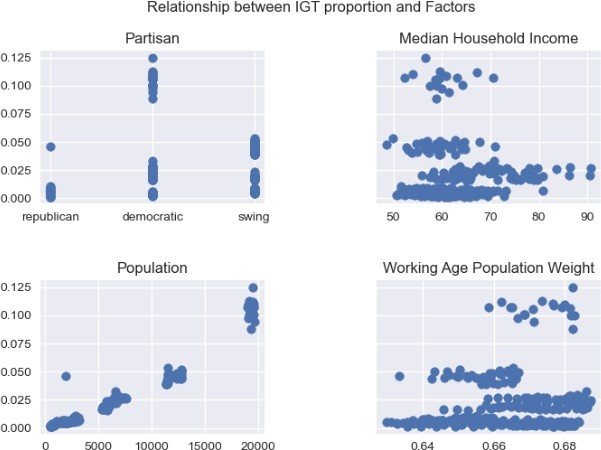
\includegraphics[scale=1]{Figures/IGT and factors.jpg}
%   \caption[IGT and Factors Scatter Plot]{Factor and IGT Scatter Plot
%     \texttt{} }
%   \label{Figure 2.3}
% \end{figure}

\subsection{Sample Collection}


I concentrate on the direct Intergovernmental Transfers (IGT) from the federal government to state governments in the United States. To integrate political influence into the data framework, I employed stratified sampling to gather samples from traditional Republican states, traditional Democratic states, and swing states.%%%%%%%%%chatgpt checked%%%%%%%


The state grouping method is based on two criteria: historical presidential election results and winning rates, following the methodology outlined in \Textcite{beachler2015presidential}'s work. Democratic states and Republican states are defined as those consistently favoring the same party in presidential elections since 1984, with winning rates exceeding 58\%. Swing states are identified as those that have chosen presidents from both parties, with winning rates below 58\%.%%%%%%%%chatgpt checked%%%%%%%

The states included in my sample are listed in Table \ref{Table 2.3}.

% Table generated by Excel2LaTeX from sheet1.
\begin{table}
  \caption{States Sample and Grouping}
  \begin{tabular}{p{7.57em}cc}
    \toprule
    States         & \multicolumn{1}{p{7.93em}}{Group}                    & \multicolumn{1}{p{6.855em}}{Code} \\
    \midrule
    Wyoming        & \multicolumn{1}{c}{\multirow{5}[2]{*}{Red States}}   & \multirow{5}[2]{*}{1}             \\
    Idaho          &                                                      &                                   \\
    Kansas         &                                                      &                                   \\
    Nebraska       &                                                      &                                   \\
    North Dakota   &                                                      &                                   \\
    \midrule
    Maryland       & \multicolumn{1}{c}{\multirow{5}[2]{*}{Blue States}}  & \multirow{5}[2]{*}{2}             \\
    Massachusetts  &                                                      &                                   \\
    Rhode Island   &                                                      &                                   \\
    New York State &                                                      &                                   \\
    Washington     &                                                      &                                   \\
    \midrule
    Pennsylvania   & \multicolumn{1}{c}{\multirow{4}[2]{*}{Swing States}} & \multirow{4}[2]{*}{3}             \\
    Nevada         &                                                      &                                   \\
    Wisconsin      &                                                      &                                   \\
    Ohio           &                                                      &                                   \\
    \bottomrule
  \end{tabular}%
  \label{Table 2.3}%
\end{table}%


The social and economic characteristics commonly included in the formula for intergovernmental transfers encompass population, working-age population weight, median household income, unemployment rate, road mileage, and GDP \parencite{dilger2015federal}. I gathered all factors mentioned in \Textcite{dilger2015federal}'s study for the sampled states. Additionally, I referenced major intergovernmental transfer programs such as Medicaid, the Title I-A education program, Temporary Assistance for Needy Families (TANF), Section 8 Housing Choice Vouchers, and the Community Development Block Grant (CDBG) to comprehensively collect factors. To ensure data convenience for regression and enhance data visualization, I performed appropriate operations. The collected characteristics and data sources are detailed in Table \ref{Table 2.4}.%%%%%%chatgpt checked%%%%%

\begin{table}
  \centering
  \caption{Social characteristics for Sample States}
  \begin{tabular}{cp{6.43em}p{9.285em}p{5.855em}p{5.355em}}
    \toprule
    \multicolumn{1}{p{4em}}{Variables } & Definition                      & Operation          & Source                              & Time Period                  \\
    \midrule
    gdp                                 & \multicolumn{1}{c}{Real GDP}    & Log transformation & FRED                                & 2000-2019 annually collected \\
    \midrule
    lgp                                 & \multicolumn{1}{c}{Population } & Log transformation & Census of bureau                    & 2000-2019 annually collected \\
    \midrule
    wapw                                & Working age population weight   & No operation       & Census of bureau                    & 2000-2019 annually collected \\
    \midrule
    mhi                                 & State median household income   & Log transformation & Census of bureau                    & 2000-2019 annually collected \\
    \midrule
    ur                                  & unemployment rate               & No operation       & FRED                                & 2000-2019 annually collected \\
    \midrule
    prm                                 & public road mileage             & Log transformation & Bureau of transportation statistics & 2000-2019 annually collected \\
    \bottomrule
  \end{tabular}%
  \label{Table 2.4}%
\end{table}%

\subsection{Descriptive Data Analysis Results}


I have conducted an analysis involving selected variables and generated scatter plots to provide an intuitive depiction of their relationships, as illustrated in Figure \ref{Figure 2.3}. The legend distinguishing different political parties has been omitted for clarity. Notably, with the exception of the lower-left subfigure depicting the relationship between "population" and "igt", which exhibits a discernible linear trend, the remaining plots reveal a pronounced hierarchical distribution.

While the linear correlation between population and intergovernmental transfer (IGT) amounts is expected, the hierarchical pattern observed across other figures is intriguing. Even when holding the x-axis constant, variations in IGT amounts persist. Particularly noteworthy is the relationship between the partisan affiliations of states and IGT amounts; for democratic states, points are dispersed on both the upper and lower sides. This hierarchical distribution suggests that social and economic characteristics alone cannot fully account for the distribution of IGT. The unexplained variance may potentially be attributed to political influences beyond legislative factors.
%%%chatgpt checked%%%%%

\begin{figure}[H]
  \centering
  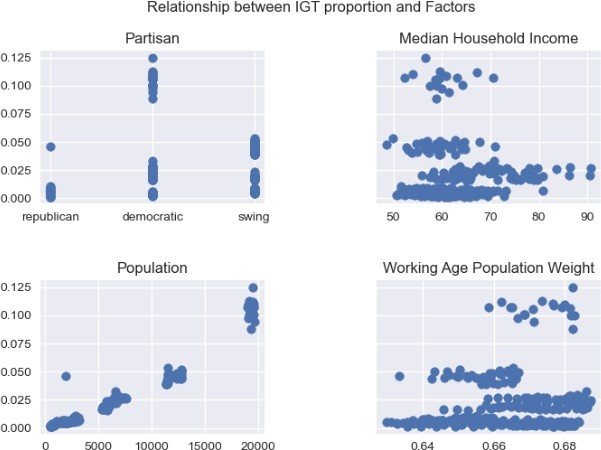
\includegraphics[scale=1]{Figures/IGT and factors.jpg}
  \caption[IGT and Factors Scatter Plot]{Factor and IGT Scatter Plot
    \texttt{} }
  \label{Figure 2.3}
\end{figure}


\section{Method Description}

The research methodology can be encapsulated from two perspectives. The first question and the rest of the questions in this paper are solved through different methods. Firstly, addressing the correlation between the free rider effect and political distribution in states necessitates an analysis of the extent of similarity among states governed by the same political party and the dissimilarity among states under different political affiliations concerning social and economic factors.

Besides, the relationship between the political factors and IGT amounts is solved through different methods.

\subsection{Method to Analyze the First Question}


As previously mentioned, the formula for distributing grants may encompass numerous factors. Additionally, issues of multicollinearity are evident within the collected variables. For example, the weight of the working-age population and the unemployment rate are highly interdependent variables and higher population levels inherently correspond to increased usage of public roads. This observation is further corroborated by the correlation heatmap, which indicates a certain degree of correlation among the variables.%%%%%chatgpt checked%%%%%

\begin{figure}
  \centering
  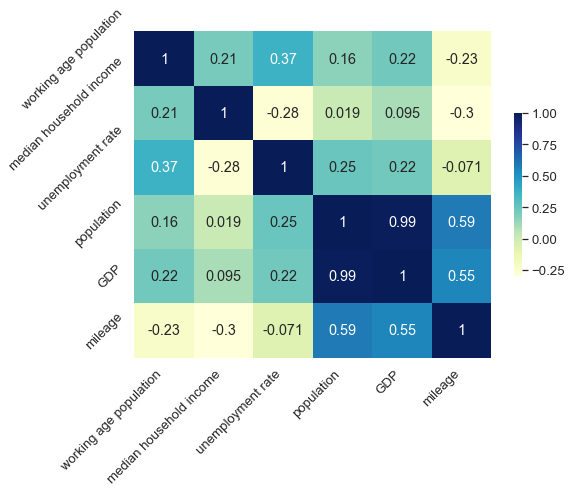
\includegraphics[scale=0.7]{Figures/heatmap.png}
  \caption[Heatmap of the Social Characteristics]{Heatmap of the Social Characteristics
    \texttt{} }
  \label{heatmap}
\end{figure}

To address the first question, the apparent hindrance lies in the difficulty of directly assessing the similarity of jurisdictions in social and economic characteristics. To overcome this challenge, I employed Principal Components Analysis (PCA) to reduce data dimensionality and mitigate issues of multicollinearity. This approach aims to determine whether the reduced-dimension data exhibit cluster distribution or scattered distribution.

The results of the PCA variance analysis, as depicted in the figure, reveal that the first two dimensions encapsulate 67\% of the information, while the first three dimensions account for 87\% of the information.
\begin{figure}[H]
  \centering  %居中
  \subfigure[Histgram]{   %第一张子图
    \begin{minipage}{7cm}
      \centering    %子图居中
      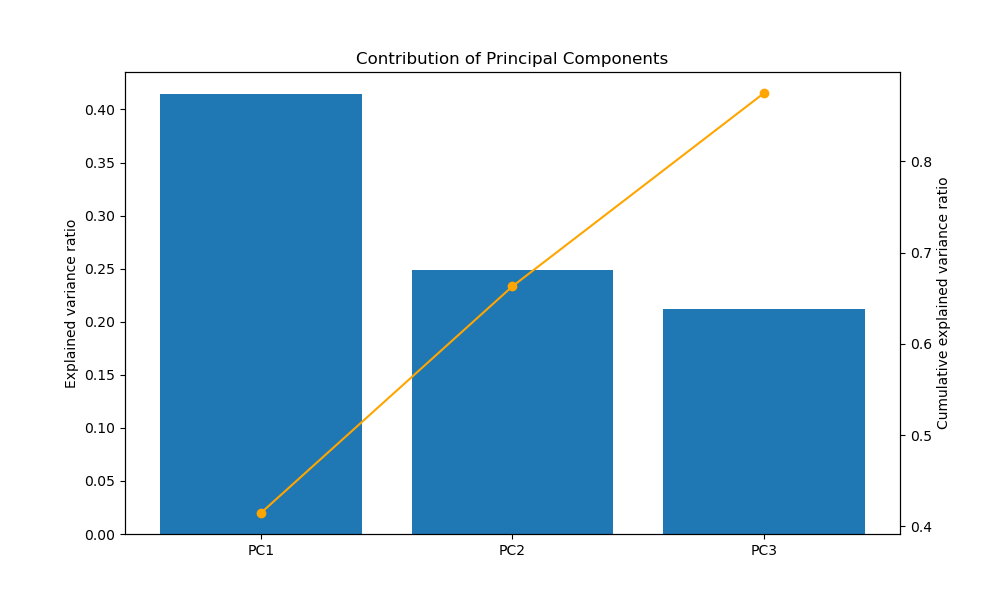
\includegraphics[scale=0.2]{Figures/contribution.png}  %以pic.jpg的0.5倍大小输出
    \end{minipage}
  }
  \subfigure[Line]{ %第二张子图
    \begin{minipage}{7cm}
      \centering    %子图居中
      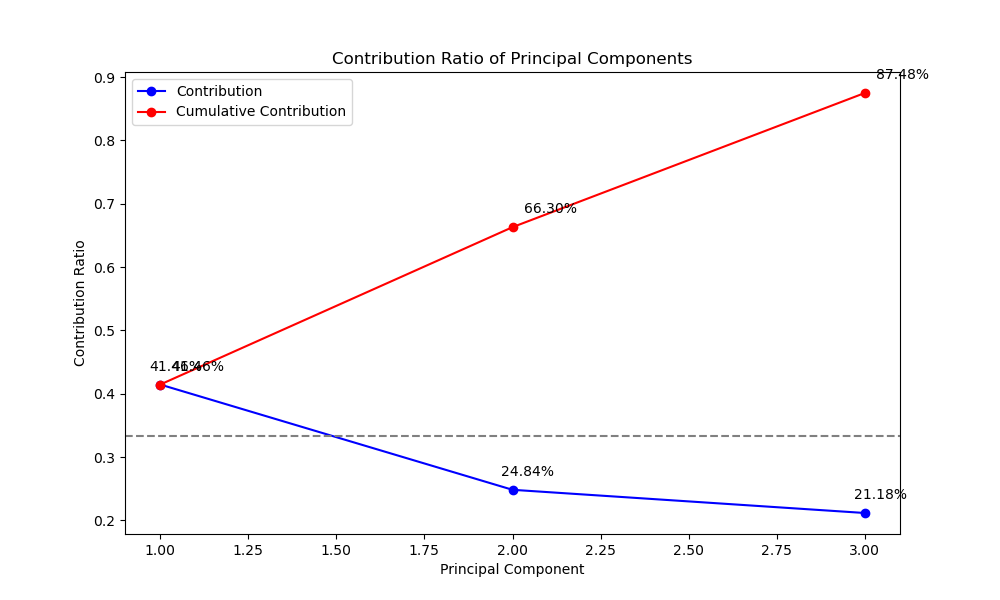
\includegraphics[scale=0.2]{Figures/contribution2.png}%以pic.jpg的0.5倍大小输出
    \end{minipage}
  }
  \caption[Principle Components Contribution]{Principle Components Contribution}    %大图名称
  \label{principlecomponentcontribution}    %图片引用标记
\end{figure}

Consequently, Principal Components Analysis (PCA) was employed to reduce the data into two and three dimensions separately. By retaining the two and three principal components with the highest information content, it became feasible to compare the characteristics between jurisdictions.

% \begin{figure}[H]
%   \centering  %居中
%   \subfigure[2 Principle Components Analysis Scatter]{   %第一张子图
%     \begin{minipage}{7cm}
%       \centering    %子图居中
%       \includegraphics[scale=0.45]{Figures/pca.png}  %以pic.jpg的0.5倍大小输出
%     \end{minipage}
%   }
%   \subfigure[3 principle Components Analysis Scatter]{ %第二张子图
%     \begin{minipage}{7cm}
%       \centering    %子图居中
%       \includegraphics[scale=0.45]{Figures/pca_3d.png}%以pic.jpg的0.5倍大小输出
%     \end{minipage}
%   }
%   \caption[Principle Components Analysis Scatter Plot]{Social Characteristics Principle Components Analysis Scatter Plot}    %大图名称
%   \label{Figure 2.2}    %图片引用标记
% \end{figure}
% %%chatgpt checked%%%%%

% Although the reduced dimensions lack specific economic meaning, a notable observation in Figure \ref{Figure 2.2} is that many state characteristics exhibit a cluster distribution. This suggests substantial similarities among jurisdictional features in the dataset. Such findings align with \Textcite{martin2018dividing}'s proposition that jurisdictions with similar features may act as free riders, consequently predicting the outflow of funds from the winning coalition.

% Another potential implication arises from the hierarchical distribution based on political parties. Republican states, Democratic states, and swing states exhibit distinct cluster distributions in their respective areas. In the 2D plot presented in Figure \ref{Figure 2.2} (a), red and blue dots are situated on opposing sides, with swing states occupying the intermediary position. This configuration implies that any modification to the grants formula favoring one party inflicts significant harm on another. This observation may elucidate the sharp opposition between the two parties during legislative bargaining, while swing states remain relatively indifferent.

% The distinctive nature of swing states is further illuminated in the 3D plot depicted in Figure \ref{Figure 2.2} (b), where green dots do not align on the same plane in the third dimension. While it is unsurprising that traditional Republican states share similar social characteristics, this figure provides an alternative perspective on any fiscal collective behavior within the party. It prompts consideration of whether members in the bargaining process act based on their political status or advocate for the benefits of their represented jurisdiction.

% This observation underscores the need to establish a micro-foundation for any collective political behavior within a party. In other words, when analyzing motivation, it is essential to focus on the motivations of individual members rather than attributing them to the entire group.
%%%%%%%%%chatgpt checked%%%%%%%%%%%%

\subsection{Regression Construction to Solve Question 2 to 5}

Despite conducting a relatively comprehensive literature review on the issue of grants distribution formulas and incorporating sample data that addresses key concerns in intergovernmental transfer distribution, the possibility remains that some variables may have been omitted from the equation, particularly given the longitudinal nature of the data spanning 19 years. Consequently, a crucial challenge in this investigation is addressing potential omitted variable issues while avoiding subsequent heteroscedasticity and endogeneity problems. To ensure unbiased estimates, I employ fixed effect model in the regression.

In the subsequent research, I present three regression models. The benchmark model is an Ordinary Least Squares (OLS) regression. Additionally, the second model is a time-factor fixed regression. The third model is a state-group variables fixed model.
%%%%%%%%%chatgpt checked%%%%%%%%%%%%


The equation for OLS regression can be displayed as follow:

\begin{equation}
  \begin{split}
    log(igt_{i,t}) & = \alpha + \beta_1 c_{i,t-1} + \beta_2 p_{i,t} + \beta_3 log(gdp) + \beta_4 log(pl) + \beta_5 log(mhi_{i,t}) \\
    & + \beta_6 wapw_{i,t} + \beta_7 ur_{i,t} +\beta_8 log(prm_{i,t}) + \epsilon_{i,t}
  \end{split}
\end{equation}
$For\ t = 1, 2, 3...T\ and\ i = 1, 2, 3...N $

The second model, which is the fixed effect model with time effect fixed is:
\begin{equation}
  \begin{split}
    log(igt_{i,t}) & = \alpha_t + \beta_1 c_{i,t-1} + \beta_2 p_{i,t} + \beta_3 log(gdp) + \beta_4 log(pl) + \beta_5 log(mhi_{i,t}) \\
    &+ \beta_6 wapw_{i,t} + \beta_7 ur_{i,t} +\beta_8 log(prm_{i,t}) + \epsilon_{i,t}
  \end{split}
\end{equation}
$For\ t = 1, 2, 3...T\ and\ i = 1, 2, 3...N $

Finally, the third model, which is states partisanship fixed effect model with state partisanship controlled is:

\begin{equation}
  \begin{split}
    log(igt_{i,t}) & = \alpha_p + \theta_t + \beta_1 c_{i,t-1} + \beta_2 p_{i,t} + \beta_3 log(gdp) + \beta_4 log(pl) + \beta_5 log(mhi_{i,t}) \\
    &+ \beta_6 wapw_{i,t} + \beta_7 ur_{i,t} +\beta_8 log(prm_{i,t}) + \epsilon_{i,t}
  \end{split}
\end{equation}
$For\ p = 0,1,2$, which stands for traditional republican states, traditional democratic states and swing states.

\subsection{Hypothesis}

There are four hypothesis in this investigation, which can be listed as follow.

\textbf{Hypothesis 1: The unified Government Hypothesis}

A unified government is characterized by the alignment of the administrative branch and legislative branch at the federal level under the same political party. This alignment tends to result in higher overall spending, as the convergence of the executive and legislative powers reduces financial constraints.

\textbf{Hypothesis 2: Party Specific Hypothesis}

The Democratic and Republican parties exhibit distinct preferences regarding the scale of Intergovernmental Transfers (IGT). The interpretation of party preferences in this context is nuanced, as two plausible inferences can be made. Concerning the government's size, the Democratic Party leans towards a larger government, leading to a higher-scale IGT. Conversely, the Republican Party holds the opposing view. When considering administrative structure, Democratic governments tend to favor a centralized system, while Republican governments prefer a decentralized structure. Consequently, these contrasting perspectives yield divergent conclusions.

\textbf{Hypothesis 3: Alignment Hypothesis}

The distribution of intergovernmental transfers (IGT) is influenced by political ideology. There is a tendency for the federal government to allocate more IGT to states controlled by the same political party.

\textbf{Hypothesis 4: Battle Ground States Hypothesis}

The level of competition between two political parties within a state has an impact on the Intergovernmental Transfers (IGT) received by that state government. The federal government, driven by the motivation to secure election or reelection, is inclined to allocate resources and provide additional public goods to states that significantly influence electoral outcomes. This strategic allocation is aimed at accruing political credits.
%%%%%%%%chatgpt checked%%%%%%%%%%%%

\section{PCA Results and Analysis}

Principal Components Analysis (PCA) was employed to reduce the data into two and three dimensions separately.The resulting scatter plot following data dimension reduction is presented in Figure \ref{Figure 2.2}.

\begin{figure}[H]
  \centering  %居中
  \subfigure[2 Principle Components Analysis Scatter]{   %第一张子图
    \begin{minipage}{7cm}
      \centering    %子图居中
      \includegraphics[scale=0.45]{Figures/pca.png}  %以pic.jpg的0.5倍大小输出
    \end{minipage}
  }
  \subfigure[3 principle Components Analysis Scatter]{ %第二张子图
    \begin{minipage}{7cm}
      \centering    %子图居中
      \includegraphics[scale=0.45]{Figures/pca_3d.png}%以pic.jpg的0.5倍大小输出
    \end{minipage}
  }
  \caption[Principle Components Analysis Scatter Plot]{Social Characteristics Principle Components Analysis Scatter Plot}    %大图名称
  \label{Figure 2.2}    %图片引用标记
\end{figure}
%%chatgpt checked%%%%%

Although the reduced dimensions lack specific economic meaning, a notable observation in Figure \ref{Figure 2.2} is that many state characteristics exhibit a cluster distribution. This suggests substantial similarities among jurisdictional features in the dataset. Such findings align with \Textcite{martin2018dividing}'s proposition that jurisdictions with similar features may act as free riders, consequently predicting the outflow of funds from the winning coalition.

Another potential implication arises from the hierarchical distribution based on political parties. Republican states, Democratic states, and swing states exhibit distinct cluster distributions in their respective areas. In the 2D plot presented in Figure \ref{Figure 2.2} (a), red and blue dots are situated on opposing sides, with swing states occupying the intermediary position. This configuration implies that any modification to the grants formula favoring one party inflicts significant harm on another. This observation may elucidate the sharp opposition between the two parties during legislative bargaining, while swing states remain relatively indifferent.

The distinctive nature of swing states is further illuminated in the 3D plot depicted in Figure \ref{Figure 2.2} (b), where green dots do not align on the same plane in the third dimension. While it is unsurprising that traditional Republican states share similar social characteristics, this figure provides an alternative perspective on any fiscal collective behavior within the party. It prompts consideration of whether members in the bargaining process act based on their political status or advocate for the benefits of their represented jurisdiction.

This observation underscores the need to establish a micro-foundation for any collective political behavior within a party. In other words, when analyzing motivation, it is essential to focus on the motivations of individual members rather than attributing them to the entire group. In the case of intergovernmental transfer, the apparent collective alliance among ostensibly similar political parties may, in reality, be attributed to the shared social and economic characteristics of their individual entities. In the process of pursuing governmental transfers for their respective interests, they may inadvertently become mutual free riders.

%%%%%%%%chatgpt checked%%%%%%%%%%%%



\section{Regression Results and Analysis}
The regression results can be summarized as Table \ref{Table 2.7}, \ref{Table 2.8} and \ref{Table 2.9}.

\begin{table}[htbp]
  \centering
  \caption{Regression Result---part 1}
  \begin{tabular}{cccc}
    \toprule
                                     & mdoel-1                      & model-2                       & model-3                      \\
                                     & OLS                          & time fixed                    & state group fixed            \\
    \midrule
    \multicolumn{1}{p{4.215em}}{c2}  & \multicolumn{1}{c}{-0.00169} & \multicolumn{1}{c}{-0.00246}  & \multicolumn{1}{c}{-0.00169} \\
                                     & (-0.52)                      & (-0.77)                       & (-0.52)                      \\
    \multicolumn{1}{p{4.215em}}{c3}  & -0.00873**                   & -0.00751*                     & -0.00873**                   \\
                                     & (-2.95)                      & (-2.49)                       & (-2.95)                      \\
    \multicolumn{1}{p{4.215em}}{c4}  & \multicolumn{1}{c}{-0.00484} & \multicolumn{1}{c}{-0.00746}  & \multicolumn{1}{c}{-0.00484} \\
                                     & (-1.21)                      & (-1.86)                       & (-1.21)                      \\
    \multicolumn{1}{p{4.215em}}{c5}  & \multicolumn{1}{c}{0.00026}  & \multicolumn{1}{c}{0.0163}    & \multicolumn{1}{c}{0.00026}  \\
                                     & \multicolumn{1}{c}{-0.06}    & \multicolumn{1}{c}{-1.39}     & \multicolumn{1}{c}{-0.06}    \\
    \multicolumn{1}{p{4.215em}}{c6}  & \multicolumn{1}{c}{0.00216}  & \multicolumn{1}{c}{0.0119}    & \multicolumn{1}{c}{0.00216}  \\
                                     & \multicolumn{1}{c}{-0.34}    & \multicolumn{1}{c}{-0.95}     & \multicolumn{1}{c}{-0.34}    \\
    \multicolumn{1}{p{4.215em}}{c7}  & -0.0107**                    & \multicolumn{1}{c}{0.000572}  & -0.0107**                    \\
                                     & (-2.80)                      & \multicolumn{1}{c}{-0.05}     & (-2.80)                      \\
    \multicolumn{1}{p{4.215em}}{c8}  & -0.00946*                    & \multicolumn{1}{c}{0.00296}   & -0.00946*                    \\
                                     & (-2.08)                      & \multicolumn{1}{c}{-0.25}     & (-2.08)                      \\
    \multicolumn{1}{p{4.215em}}{c9}  & -0.00676**                   & \multicolumn{1}{c}{0.00384}   & -0.00676**                   \\
                                     & (-3.31)                      & \multicolumn{1}{c}{-1.07}     & (-3.31)                      \\
    \multicolumn{1}{p{4.215em}}{c10} & \multicolumn{1}{c}{-0.00588} & \multicolumn{1}{c}{-0.000158} & \multicolumn{1}{c}{-0.00588} \\
                                     & (-1.43)                      & (-0.04)                       & (-1.43)                      \\
    \multicolumn{1}{p{4.215em}}{c11} & \multicolumn{1}{c}{0.000423} & \multicolumn{1}{c}{0.00893}   & \multicolumn{1}{c}{0.000423} \\
                                     & \multicolumn{1}{c}{-0.05}    & \multicolumn{1}{c}{-1.11}     & \multicolumn{1}{c}{-0.05}    \\
    \multicolumn{1}{p{4.215em}}{c12} & -0.00898*                    & \multicolumn{1}{c}{0}         & -0.00898*                    \\
                                     & (-2.44)                      & (.)                           & (-2.44)                      \\
    \bottomrule
  \end{tabular}%
  \label{Table 2.7}%
\end{table}%


% Table generated by Excel2LaTeX from sheet 'Sheet1'
\begin{table}[htbp]
  \centering
  \caption{Regression Result---part 2}
  \begin{tabular}{llll}
    \toprule
                                                        & \multicolumn{1}{p{7.93em}}{mdoel-1} & \multicolumn{1}{p{7.855em}}{model-2}     & \multicolumn{1}{p{7.855em}}{model-3}           \\
                                                        & \multicolumn{1}{p{7.93em}}{OLS}     & \multicolumn{1}{p{7.855em}}{time fixed } & \multicolumn{1}{p{7.855em}}{state group fixed} \\
    \midrule
    \multicolumn{1}{p{8.355em}}{c13}                    & -0.00083                            & 0.00919                                  & -0.00083                                       \\
                                                        & \multicolumn{1}{p{7.93em}}{(-0.20)} & -1.74                                    & \multicolumn{1}{p{7.855em}}{(-0.20)}           \\
    \multicolumn{1}{p{8.355em}}{c14}                    & -0.00223                            & -0.000932                                & -0.00223                                       \\
                                                        & \multicolumn{1}{p{7.93em}}{(-0.32)} & \multicolumn{1}{p{7.855em}}{(-0.14)}     & \multicolumn{1}{p{7.855em}}{(-0.32)}           \\
    \multicolumn{1}{p{8.355em}}{c15}                    & -0.0136                             & -0.00713                                 & -0.0136                                        \\
                                                        & \multicolumn{1}{p{7.93em}}{(-2.34)} & \multicolumn{1}{p{7.855em}}{(-1.15)}     & \multicolumn{1}{p{7.855em}}{(-2.34)}           \\
    \multicolumn{1}{p{8.355em}}{c16}                    & -0.006                              & 0                                        & -0.006                                         \\
                                                        & \multicolumn{1}{p{7.93em}}{(-1.40)} & \multicolumn{1}{p{7.855em}}{(.)}         & \multicolumn{1}{p{7.855em}}{(-1.40)}           \\
    \multicolumn{1}{p{8.355em}}{Democratic}             & -0.00585                            & -0.0125                                  & 0                                              \\
                                                        & \multicolumn{1}{p{7.93em}}{(-1.24)} & \multicolumn{1}{p{7.855em}}{(-2.60)}     & \multicolumn{1}{p{7.855em}}{(.)}               \\
    \multicolumn{1}{p{8.355em}}{Swing}                  & -0.0175                             & -0.0224                                  & 0                                              \\
                                                        & \multicolumn{1}{p{7.93em}}{(-5.90)} & \multicolumn{1}{p{7.855em}}{(-7.21)}     & \multicolumn{1}{p{7.855em}}{(.)}               \\
    \multicolumn{1}{p{8.355em}}{Log(population)}        & -0.0569                             & -0.0548                                  & -0.0569                                        \\
                                                        & \multicolumn{1}{p{7.93em}}{(-5.42)} & \multicolumn{1}{p{7.855em}}{(-4.46)}     & \multicolumn{1}{p{7.855em}}{(-5.42)}           \\
    \multicolumn{1}{p{8.355em}}{working age population} & 0.0848                              & \multicolumn{1}{p{7.855em}}{0.318**}     & 0.0848                                         \\
                                                        & -1.2                                & -3.21                                    & -1.2                                           \\
    \bottomrule
  \end{tabular}%
  \label{Table 2.8}%
\end{table}%

% Table generated by Excel2LaTeX from sheet 'Sheet1'
\begin{table}[htbp]
  \centering
  \caption{Regression Result---part 3}
  \begin{tabular}{p{9.285em}lll}
    \toprule
    \multicolumn{1}{c}{}    & \multicolumn{1}{p{7.645em}}{mdoel-1}    & \multicolumn{1}{p{8.57em}}{model-2}     & \multicolumn{1}{p{7.145em}}{model-3}           \\
    \multicolumn{1}{c}{}    & \multicolumn{1}{p{7.645em}}{OLS}        & \multicolumn{1}{p{8.57em}}{time fixed } & \multicolumn{1}{p{7.145em}}{state group fixed} \\
    \midrule
    median household income & \multicolumn{1}{p{7.645em}}{-0.284***}  & \multicolumn{1}{p{8.57em}}{-0.311***}   & \multicolumn{1}{p{7.145em}}{-0.284***}         \\
    \multicolumn{1}{r}{}    & \multicolumn{1}{p{7.645em}}{(-15.24)}   & \multicolumn{1}{p{8.57em}}{(-16.06)}    & \multicolumn{1}{p{7.145em}}{(-15.24)}          \\
    unemployment rate       & \multicolumn{1}{p{7.645em}}{-0.00166**} & -0.000939                               & \multicolumn{1}{p{7.145em}}{-0.00166**}        \\
    \multicolumn{1}{r}{}    & \multicolumn{1}{p{7.645em}}{(-2.79)}    & \multicolumn{1}{p{8.57em}}{(-1.13)}     & \multicolumn{1}{p{7.145em}}{(-2.79)}           \\
    Log(GDP)                & \multicolumn{1}{p{7.645em}}{0.126***}   & \multicolumn{1}{p{8.57em}}{0.129***}    & \multicolumn{1}{p{7.145em}}{0.126***}          \\
    \multicolumn{1}{r}{}    & -11.73                                  & -10.65                                  & -11.73                                         \\
    Log(mileage)            & \multicolumn{1}{p{7.645em}}{-0.0180***} & \multicolumn{1}{p{8.57em}}{-0.0231***}  & \multicolumn{1}{p{7.145em}}{-0.0180***}        \\
    \multicolumn{1}{r}{}    & \multicolumn{1}{p{7.645em}}{(-4.09)}    & \multicolumn{1}{p{8.57em}}{(-5.22)}     & \multicolumn{1}{p{7.145em}}{(-4.09)}           \\
    Constant                & \multicolumn{1}{p{7.645em}}{0.123*}     & 0.018                                   & \multicolumn{1}{p{7.145em}}{0.116*}            \\
    \multicolumn{1}{r}{}    & -2.29                                   & -0.3                                    & -2.14                                          \\
    \midrule
    Observations            & 294                                     & 294                                     & 294                                            \\
    Adjusted R2             & 0.835                                   & 0.845                                   & 0.79                                           \\
    \bottomrule
  \end{tabular}%
  \label{Table 2.9}%
\end{table}%

The initial observation in the presentation indicates that all three models exhibit high adjusted $R^2$. The elevated adjusted $R^2$ values can be attributed to the substantial explanatory power of the selected control variables.

In the third model, where state partisanship variables are fixed and the sample selection criteria ensure partisan stability over the past 19 years, the deduction process in fixed effect regression results in the omission of the partisan variable. This accounts for the coefficients of partisan variables being zero.

For subsequent analyses, I will utilize the coefficients of partisanship variables of states (democratic, republican and swing) from model 2 and incorporate all other coefficients from model 3. The reason is that, 19 years is not a long time, especially the data is annually collected. In such a short period, significant shifts in governing styles or political environments, regardless of party affiliation, are unlikely to occur. The fixed regression on state groups in terms of the partisan is relatively reasonable.

%%%%%%%chatgpt checked%%%%%%%%%%%%

In model 3, the coefficients $c_3(r, r, d, r),c_7(r, d, d, r),c_8(r, d, d, d),c_9(d, r, r, r),c_{12}(d, r, d, d),c_{15}(d, d, d, r)$ are statistically significant at 5\% significance level. Similarly, in model 2, the partisan variables "Democratic States" and "Swing States" also exhibit significance.
%%%%%chatgpt checked%%%%%%%%%%%%

The regression results support the first hypothesis concerning unified government. A comparison between the coefficient of $c_9(d, r, r, r)$ and $c_1(r, r, r, r)$ reveals that a traditional Republican state, where both the administrative and legislative branches are controlled by the Republican party, experiences a 0.67\% reduction in intergovernmental transfers under bipartisan control at the federal level compared to a situation where the federal government is uniformly controlled by the republican party. This suggests that the ability to distribute grants to the state level is significantly constrained when the Republican party does not have unified control at the federal level.
%%%chatgpt checked%%%%%


Upon comparing the coefficient of $c_{16}(d, d, d, d)$ and $c_1(r, r, r, r)$, it is evident that states receive a 0.6\% lower intergovernmental transfer when both the federal and state levels are controlled by the Democratic party, in contrast to a scenario where both levels are under Republican control. This implies a republican party preference for allocating more resources to state governments, aligning with the primary inference in my hypothesis. However the coefficient of $c_{16}$ is not significant thus we cannot null hypothesis that that there is no difference between $c_1$ and $c_{16}$ and hypothesis 2 is not supported.

%%%chatgpt checked%%%%%

The alignment effect proves to be statistically significant in the distribution of intergovernmental transfers. When comparing the aligned combination $c_1(r, r, r, r)$ and $c_3(r, r, d, r)$, the negative coefficient of $c_3$ indicates that unaligned states with a Republican-controlled federal government would receive fewer grants. Specifically, aligned Republican states receive 0.87\% more grants compared to states with a Democratic governor\footnote{Massive negative coefficients of $c$ combinations further underscore the significance of the alignment effect.}.

In conclusion, regarding the impact of state partisanship, the coefficient of swing states in model 2 suggests that swing states receive fewer grants compared to both Republican and Democratic states. One plausible explanation is that swing states experience increased funding only during election periods. While theoretical analysis and supporting literature highlight the benefits swing states receive during elections, this longitudinal study spanning 19 years suggests that in non-election years, when politicians are less concerned about electoral pressure and political credit, the motivation to garner support from swing states diminishes.

\section{Review and Summary}

I acknowledge the limitations and deficiencies in this investigation. The most apparent drawback is the limited time span of the data, which might be more significant considering that elections occur every two or even four years, not annually. It could be argued that our model lacks robustness, as our conclusions may not maintain validity when extended to a longer time span.

Another deficiency is the explain of the coefficients of the partisan combination variables $c$. The statistical result can give us the observation of behavior, but tells barely about the motivation of the behavior. In this regression analysis, though we get some evidence to support the hypothesis I proposed, we don't capture the motivation accurately. For example, the compare between the coefficients of $c_1$ and $c_3$ support the hypothesis on alignment. However when the bargaining process happens in central level, are the members of committee care about the states with same partisan? or they just care about the specific state and other states share similar social and economic features became free riders? From the PCA analysis, we just cannot deny the latter.

Moreover, I employed the total amounts of Intergovernmental Transfers (IGT) received by states as dependent variables, indicating that I did not distinguish between competitive grants and formula grants in the regression. Besides considerations of convenience, this choice was influenced by the fact that formula grants constitute the majority of the total grant amounts. However, I acknowledge that these two types of grants should be differentiated. For instance, the free rider effect may not be significant in competitive grants, as decision-making groups at the central level can manipulate the amounts received in the competitive grants process, while they can only influence variables in the formula grants.

This paper also serves as an extension that may provide insights into related areas. This research serves as supplementary material for the flypaper effect. The flypaper effect posits that an increase in grants-in-aid leads to significantly higher public spending compared to the same increase in private income, causing funds to "stick where they hit" \parencite{inman2008flypaper}. Scholars attribute this phenomenon to various causes. Hamilton, for instance, attempted to explain the flypaper effect as a result of improper data distinction or empirical methods \parencite{hamilton1986flypaper}. Others associate the flypaper effect with fiscal illusion \parencite{gramlich1997stimulative}.

This research introduces a novel perspective to comprehend the flypaper effect. The confirmed biased effect in grants distribution suggests that, for certain states, obtaining grants from the federal government is easier compared to generating revenue through other means. This relative price effect may explain the inclination of state governments to prefer raising funds from Intergovernmental Transfers (IGT) rather than through taxation. Following this logic, the magnitude of the flypaper effect should be influenced by the partisan distribution between the central and state governments. States that are prone to free-riding or are favored by central governments may experience a greater flypaper effect, as grants for such subnational entities are relatively easier to obtain, amplifying their spending tendencies.

% One potential extension for this research is to evaluate the impact of $c$ in competitive grants and formula grants separately.


%%%chatgpt checked%%%%%
% The examination of Intergovernmental Transfers (IGT) is situated within the framework of fiscal federalism. While fiscal federalism offers various benefits, as noted by \Textcite{musgrave1971economics}, it also presents several challenges. Our investigation may offer implications for explaining some of the problems.

%%%%%%%%%
% One such challenge is the manifestation of loss aversion behavior between national and subnational governments \parencite{alesina2019loss, bourdeaux2018loss, rees2014loss}. Loss aversion arises due to the subnational entities being less accountable for the separation of funding and spending responsibilities in local government. This introduces information asymmetry \parencite{brennan1987efficient, huber2006optimal, miller1985dividend}, posing risks to the allocative efficiency of federal spending. Issues such as conflict of interest and moral hazard may compromise the effectiveness of federal spending. For instance, moral hazard problems may discourage subnational governments from cost-effectively delivering services \parencite{williams2021moral}, resulting in shirking behavior.
%%%%%%%感觉有点驴唇不对马嘴,得想一想怎么才能更好的嵌入进文章当中去。

% Furthermore, the delegation of program implementation from a central government to a subnational government increases information asymmetry, potentially exacerbating the incentive problems discussed earlier. This delegation may also elevate the risk of agents within a subnational government engaging in behaviors inconsistent with program goals, leading to conflicts of interest problems. Our analysis offers some potential explanations.

% The investigation confirms the impact of political party bias on grants distribution, a phenomenon likely known to both federal and state governments. Once state governments are assured of the grants they receive, their motivation to diligently implement policies may decrease. Therefore, the incentive problem can be partially attributed to the biased grants distribution process.

% Finally, 

\printbibliography

\appendix
\section{Data}

\begin{table}
  \centering
  \caption{Data Source and operation for the empirical test in Section 2.3.3}
  \begin{tabular}{ccp{8.785em}c}
    \toprule
    \multicolumn{2}{p{13.93em}}{Variables }                                         & Source  & \multicolumn{1}{p{7.785em}}{Time Period}                                                                         \\
    \midrule
    \multicolumn{1}{p{7em}}{Dependent Variable}                                     & lg(igt) & State CAFR                               & \multicolumn{1}{c}{\multirow{9}[18]{*}{2000-2019 annually collected}} \\
    \cmidrule{1-3}    \multicolumn{1}{c}{\multirow{2}[4]{*}{Independent Variables}} & c       & \multirow{2}[4]{*}{Ballotpedia}          &                                                                       \\
    \cmidrule{2-2}                                                                  & p       & \multicolumn{1}{c}{}                     &                                                                       \\
    \cmidrule{1-3}    \multicolumn{1}{c}{\multirow{6}[12]{*}{Control Variables}}    & gdp     & FRED                                     &                                                                       \\
    \cmidrule{2-3}                                                                  & lgp     & \multirow{4}[8]{*}{Census of bureau}     &                                                                       \\
    \cmidrule{2-2}                                                                  & wapw    & \multicolumn{1}{c}{}                     &                                                                       \\
    \cmidrule{2-2}                                                                  & mhi     & \multicolumn{1}{c}{}                     &                                                                       \\
    \cmidrule{2-2}                                                                  & ur      & \multicolumn{1}{c}{}                     &                                                                       \\
    \cmidrule{2-3}                                                                  & prm     & Bureau of transportation statistics      &                                                                       \\
    \bottomrule
  \end{tabular}%
  \label{Table A.1}%
\end{table}%

\end{document}

%% 
%% Copyright (C) 2019 by Daniel A. Weiss <daniel.weiss.led at gmail.com>
%% 
%% This work may be distributed and/or modified under the
%% conditions of the LaTeX Project Public License (LPPL), either
%% version 1.3c of this license or (at your option) any later
%% version.  The latest version of this license is in the file:
%% 
%% http://www.latex-project.org/lppl.txt
%% 
%% Users may freely modify these files without permission, as long as the
%% copyright line and this statement are maintained intact.
%% 
%% This work is not endorsed by, affiliated with, or probably even known
%% by, the American Psychological Association.
%% 
%% This work is "maintained" (as per LPPL maintenance status) by
%% Daniel A. Weiss.
%% 
%% This work consists of the file  apa7.dtx
%% and the derived files           apa7.ins,
%%                                 apa7.cls,
%%                                 apa7.pdf,
%%                                 README,
%%                                 APA7american.txt,
%%                                 APA7british.txt,
%%                                 APA7dutch.txt,
%%                                 APA7english.txt,
%%                                 APA7german.txt,
%%                                 APA7ngerman.txt,
%%                                 APA7greek.txt,
%%                                 APA7czech.txt,
%%                                 APA7turkish.txt,
%%                                 APA7endfloat.cfg,
%%                                 Figure1.pdf,
%%                                 shortsample.tex,
%%                                 longsample.tex, and
%%                                 bibliography.bib.
%% 
%%
%% End of file `./samples/longsample.tex'.
